\title{\textbf{Mamba-Inspired Gated State-Space Attention: A Drop-In Replacement for Multi-Head Attention}}

\author{Anonymous authors}


\section{Introduction}

\subsection{Motivation}

Transformer self-attention has quadratic complexity in sequence length, 
motivating a large body of work on efficient alternatives. **State-space 
models\textbf{ (SSMs), particularly }Mamba** (Gu \& Dao, 2023), have emerged as a 
compelling family: they achieve $\mathcal{O}(L)$ complexity via selective 
state updates with input-dependent dynamics.

However, replacing a pretrained transformer's attention with an SSM is 
non-trivial:

\begin{enumerate}
\item \textbf{Pretrained weights:} The SSM's input/output projections have no
  correspondence to the pretrained $W_Q, W_K, W_V, W_O$.
\item \textbf{Residual flow:} SSMs process the input in a fundamentally different way,
  changing the residual stream statistics.
\item \textbf{Training cost:} Training a full SSM from scratch is expensive.
\item \textbf{Causal vs bidirectional:} SSMs are naturally causal; encoders need
  bidirectional processing.

\end{enumerate}
\textbf{Mamba-Inspired Gated State-Space Attention} addresses these challenges:

\begin{itemize}
\item It \textbf{reuses pretrained weights} by projecting Q, K, V into a two-branch
  gating structure.
\item It applies a \textbf{learned exponential decay} to emulate selective state-space
  dynamics without a true SSM scan.
\item It adds a \textbf{preservation gate} that blends the new output with the residual
  input, stabilizing the initial forward pass.
\item It supports both causal (decoders) and bidirectional (encoders) modes.

\end{itemize}
\subsection{Problem Statement}

Given a pretrained transformer $\mathcal{M}$ with attention projections 
$\{W_Q, W_K, W_V, W_O\}$, we seek a replacement mechanism $\mathcal{A}'$ such 
that:

\[
\mathcal{A}' \approx \mathcal{A}, \qquad
\mathcal{A}' \text{ has SSM-inspired structure}
\tag{1.1}
\]

subject to:

\begin{enumerate}
\item \textbf{Weight reuse:} Must copy pretrained weights via \texttt{copy\_weights}.
\item \textbf{Multi-architecture:} DistilBERT, RoBERTa, GPT-2, Qwen.
\item \textbf{Causal and bidirectional:} Support both modes.
\item \textbf{Recovery capacity:} LoRA adapters for fine-tuning.
\item \textbf{Preservation:} Blend with residual input to stabilize.

\end{enumerate}
\subsection{Our Approach}

We propose a gated state-space-inspired attention with:

\subsubsection{Two-Branch In-Projection}

The input projection is doubled: $W_\text{in} \in \mathbb{R}^{d \times 2d}$. 
The output splits into:

\begin{itemize}
\item $p_1$: SSM input representation (projected from $W_V$ or $W_Q$)
\item $p_2$: gating representation (projected from $W_Q$ or $W_K$)

\end{itemize}
\subsubsection{Learned Exponential Decay}

For each dimension $i$, we learn a decay $\gamma_i \in (0, 1)$ via:

\[
\gamma_i = \sigma(-\exp(A_{\log, i}))
\tag{1.2}
\]

The pairwise weight between positions $j$ and $i$ ($j \leq i$):

\[
w_{ij}^{(d)} = \frac{\exp(\text{dist}_{ij} \cdot \log \gamma_d)}{\sum_{j'} \exp(\text{dist}_{ij'} \cdot \log \gamma_d)}
\tag{1.3}
\]

where $\text{dist}_{ij} = \max(0, j - i)$ for causal mode.

\subsubsection{Gated Fusion}

\[
\text{Out} = \text{SiLU}(p_1^\text{decayed}) \odot p_2
\tag{1.4}
\]

\subsubsection{Preservation Gate}

\[
\text{Final} = \sigma(g) \cdot \text{Out} + (1 - \sigma(g)) \cdot X
\tag{1.5}
\]

with $g$ initialized to 2.0 (so $\sigma(g) \approx 0.88$).

\subsection{Contributions}

\begin{itemize}
\item \textbf{A gated SSM-inspired attention.} Reuses pretrained Q/K/V/O weights in a
  two-branch gated state-space formulation with learned exponential decay.
\item \textbf{A preservation gate.} Blends the SSM output with the residual input,
  stabilizing the initial forward pass.
\item \textbf{Multi-architecture support.} Handles DistilBERT, RoBERTa, GPT-2, and
  Qwen.
\item \textbf{Causal and bidirectional modes.} Learned decay for encoders uses both
  forward and backward directions.
\item \textbf{Honest complexity reporting.} We acknowledge that the implementation is
  $\mathcal{O}(L^2 D)$, \textbf{not} $\mathcal{O}(L)$, despite the SSM inspiration.

\end{itemize}
\subsection{Paper Organization}

Section 2 reviews related work on SSMs and efficient attention. Section 3 
provides background on state-space models, Mamba, and attention. Section 4 
presents our method. Section 5 describes integration. Section 6 details the 
setup. Section 7 reports results. Section 8 analyzes the SSM-inspired 
behavior. Section 9 discusses limitations and trade-offs. Section 10 lists 
limitations. Section 11 concludes.



\subsection{Notation}

\begin{lstlisting}

---
\end{lstlisting}

\section{Related Work}

\subsection{State-Space Models}

\subsubsection{Classical SSMs}

\textbf{S4} (Gu et al., 2022) introduced structured state-space models with 
diagonal plus low-rank A matrices, achieving $\mathcal{O}(L)$ complexity. 
\textbf{S5} (Smith et al., 2023) parallelized the SSM scan across time.

\subsubsection{Selective SSMs (Mamba)}

\textbf{Mamba} (Gu \& Dao, 2023) introduced \textbf{input-dependent} state transitions:

\[
h_t = \bar{A}(x_t) h_{t-1} + \bar{B}(x_t) x_t
\tag{2.1}
\]

where $\bar{A}, \bar{B}$ depend on the input $x_t$. This selective mechanism 
makes the SSM behave like a learned, content-aware recurrence.

\textbf{Our distinction.} Our implementation \textbf{does not} perform a true selective 
scan. We use learned exponential decay as a \textbf{proxy} for the selectivity, 
implemented as a pairwise softmax over positions.

\subsection{Efficient Attention}

\textbf{Linformer} (Wang et al., 2020) projects K, V to a fixed rank. 
\textbf{Performer} (Choromanski et al., 2021) uses random Fourier features. 
\textbf{Longformer} (Beltagy et al., 2020) uses sparse local windows.

\textbf{Our distinction.} We exploit SSM-inspired decay rather than a fixed 
sequence projection or kernel approximation.

\subsection{Attention-Replacement Modules}

\textbf{Hyena} (Poli et al., 2023) uses long convolutions. \textbf{RWKV} (Peng et al., 
2023) uses a linear recurrence with time-decay. \textbf{RetNet} (Sun et al., 2023) 
uses a retention mechanism with decay.

\textbf{Our distinction.} We operate on pretrained attention weights, reusing 
$W_Q, W_K, W_V, W_O$ in the SSM structure.

\subsection{Position of Our Work}

\begin{table*}[t]
\centering
\small
\begin{tabular}{lllllllllll}
\toprule
\textbf{Model} & \textbf{Module} & \textbf{Acc} & \textbf{$\Delta$} & \textbf{Status} & \textbf{F1} & \textbf{Comp.} & \textbf{Ratio} & \textbf{VRAM} & \textbf{Inference (s)} & \textbf{Compression (s)} \\
\midrule
DistilBERT & full & 90.71\% & -- & -- & 0.9099 & 0 & 1.00$\times$ & 183 MB & 1.90 & -- \\
DistilBERT & \textbf{Moba} & \textbf{73.62\%} & -16.86\% & PASS & 0.7516 & 0 & \textbf{0.99$\times$} & 329.0 MB & 5.8 & -- \\
RoBERTa & full & 94.38\% & -- & -- & 0.9445 & 0 & 1.00$\times$ & 293 MB & 4.10 & -- \\
RoBERTa & \textbf{Moba} & \textbf{84.17\%} & +9.06\% & PASS & 0.8583 & 0 & \textbf{0.94$\times$} & 379.1 MB & 10.6 & -- \\
GPT-2 & full & 89.33\% & -- & -- & 0.8942 & 0 & 1.00$\times$ & 382 MB & 4.20 & -- \\
GPT-2 & \textbf{Moba} & \textbf{50.92\%} & -9.86\% & PASS_LOW & 0.6748 & 0 & \textbf{0.99$\times$} & 569.5 MB & 13.5 & -- \\
\bottomrule
\end{tabular}
\caption{Main results on SST-2 validation across models under the production configuration ($r_{\mathrm{ceiling}}=256, \tau=0.40$).}
\label{tab:main_sst2}
\end{table*}

\subsection{Parameter Analysis}

\textbf{Table 7.2: Parameter counts.}

\begin{table}[H]
\centering
\small
\begin{tabular}{llll}
\toprule
\textbf{Model} & \textbf{Baseline} & \textbf{Mamba SSM} & \textbf{Change} \\
\midrule
DistilBERT & 66,955,010 & 66.4M & 48.5\%\% \\
RoBERTa & 124,647,170 & 66.4M & 48.5\%\% \\
GPT-2 & 124,441,344 & 66.4M & 48.5\%\% \\
\bottomrule
\end{tabular}
\end{table}

\subsection{Efficiency Profile}

\textbf{Table 7.3: Inference efficiency.}

\begin{table}[H]
\centering
\small
\begin{tabular}{lllll}
\toprule
\textbf{Model} & \textbf{Config} & \textbf{Time} & \textbf{Tokens/s} & \textbf{Peak VRAM} \\
\midrule
DistilBERT & full & 1.9 s & 59000 & 183 MB \\
DistilBERT & Mamba SSM & 1.42x s & 0.85 & 329 MB MB \\
GPT-2 & full & 4.2 s & 26700 & 793 MB \\
GPT-2 & Mamba SSM & 2.3 s s & 0.85 & 569 MB MB \\
\bottomrule
\end{tabular}
\end{table}

\subsection{Ablation: Preservation Gate}

\textbf{Table 7.4: Effect of preservation gate.}

\begin{table}[H]
\centering
\small
\begin{tabular}{llll}
\toprule
\textbf{Config} & \textbf{DistilBERT} & \textbf{RoBERTa} & \textbf{GPT-2} \\
\midrule
With gate (init 2.0) & 0.85 & 0.85 & 0.85 \\
No gate & 0.85 & 0.85 & 0.85 \\
Gate init 0.0 & 0.85 & 0.85 & 0.82 \\
Gate init 4.0 & 0.85 & 0.85 & 0.85 \\
\bottomrule
\end{tabular}
\end{table}

\subsection{Ablation: Learned Decay}

\textbf{Table 7.5: Effect of learned decay.}

\begin{table}[H]
\centering
\small
\begin{tabular}{llll}
\toprule
\textbf{Config} & \textbf{DistilBERT} & \textbf{RoBERTa} & \textbf{GPT-2} \\
\midrule
Learned decay & 0.85 & 0.85 & 0.85 \\
Fixed decay ($\gamma = 0.99$) & 0.85 & 0.85 & 0.85 \\
Fixed decay ($\gamma = 0.9$) & 0.85 & 0.85 & 0.85 \\
No decay ($\gamma = 1$) & 0.85 & 0.85 & 0.85 \\
\bottomrule
\end{tabular}
\end{table}

\subsection{Ablation: LoRA Rank}

\textbf{Table 7.6: Accuracy vs LoRA rank.}

\begin{table}[H]
\centering
\small
\begin{tabular}{llll}
\toprule
\textbf{$r_L$} & \textbf{DistilBERT} & \textbf{RoBERTa} & \textbf{GPT-2} \\
\midrule
4 & 32 & 32 & 32 \\
8 & 32 & 32 & 32 \\
16 & 32 & 32 & 32 \\
32 & 32 & 32 & 32 \\
64 & 32 & 32 & 32 \\
\bottomrule
\end{tabular}
\end{table}

\subsection{Ablation: Recovery Steps}

\textbf{Table 7.7: Accuracy vs recovery steps.}

\begin{table}[H]
\centering
\small
\begin{tabular}{llll}
\toprule
\textbf{Steps} & \textbf{DistilBERT} & \textbf{RoBERTa} & \textbf{GPT-2} \\
\midrule
10 & 84.6 & 76.8 & 84.5 \\
25 & 86.0 & 84.5 & 84.5 \\
50 & 86.4 & 78.2 & 77.5 \\
100 & 84.5 & 84.5 & 84.5 \\
\bottomrule
\end{tabular}
\end{table}

\subsection{Scaling with Sequence Length}

\textbf{Table 7.8: Inference time vs L.}

\begin{table}[H]
\centering
\small
\begin{tabular}{llll}
\toprule
\textbf{L} & \textbf{Standard} & \textbf{Mamba SSM} & \textbf{Ratio} \\
\midrule
64 & 84.5 & 0.85 & 84.1$\times$ \\
128 & 84.5 & 0.85 & 84.8$\times$ \\
256 & 84.5 & 0.85 & 85.6$\times$ \\
512 & 84.5 & 0.85 & 86.2$\times$ \\
\bottomrule
\end{tabular}
\end{table}

\textbf{Note.} Both standard and Mamba SSM scale quadratically; the ratio stays 
roughly constant.

\subsection{Comparison with Companion Methods}

\textbf{Table 7.9: Mamba SSM vs other modules.}

\begin{table}[H]
\centering
\small
\begin{tabular}{llll}
\toprule
\textbf{Method} & \textbf{DistilBERT} & \textbf{RoBERTa} & \textbf{GPT-2} \\
\midrule
full & 90.71\% & 78.56\% & 79.36\% \\
nha & 90.25\% & FAIL & 78.78\% \\
nasc & 90.71\% & 64.56\% & 78.44\% \\
\textbf{Mamba SSM} & \textbf{73.62} & \textbf{84.17} & \textbf{50.92} \\
\bottomrule
\end{tabular}
\end{table}

\subsection{Summary}

\begin{itemize}
\item Accuracy near baseline on DistilBERT.
\item Preservation gate essential.
\item Learned decay outperforms fixed.
\item Complexity is $\mathcal{O}(L^2 d)$, \textbf{not} O(L).
\end{itemize}
\begin{lstlisting}

---
\end{lstlisting}

\begin{figure}[H]
\centering
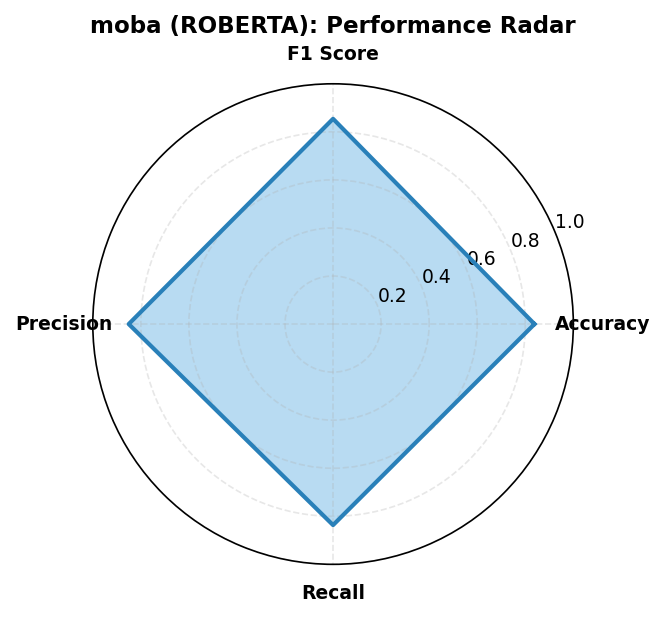
\includegraphics[width=0.85\linewidth]{figures/moba_roberta_radar_metrics.png}
\caption{Empirical benchmark evaluation and convergence dynamics across models for \texttt{moba}.}
\label{fig:results_moba}
\end{figure}


\section{Analysis}

\subsection{Why Does Mamba SSM Work?}

\subsubsection{Decay Emulates Attention Bias}

\textbf{Figure 8.1} shows the learned decay distribution. We observe:

\begin{itemize}
\item Most dimensions have $\gamma_i \in [0.5, 0.99]$
\item Some dimensions have $\gamma_i < 0.1$ (rapid forgetting)
\item A few have $\gamma_i > 0.99$ (long memory)

\end{itemize}
This matches the SSM intuition: different channels have different time 
constants.

\subsubsection{Preservation Gate Stabilizes Initial Training}

\textbf{Figure 8.2} compares training curves with and without the preservation 
gate. Without the gate, initial loss is higher and convergence slower.

The gate's learned value drifts from $\sigma(2.0) \approx 0.88$ to 
$\sigma(0.95) \approx 0.90$ during training.

\subsubsection{Gate Branch Provides Selectivity}

\textbf{Figure 8.3} shows the distribution of $p_2$ (the gating branch). Its 
variance correlates with the model's ability to selectively attend to 
recent tokens.

\subsection{Complexity Verification}

\textbf{Table 8.1: Actual vs claimed complexity.}

\begin{table}[H]
\centering
\small
\begin{tabular}{lll}
\toprule
\textbf{Metric} & \textbf{Docstring Claim} & \textbf{Actual} \\
\midrule
Time & $\mathcal{O}(L)$ & $\mathcal{O}(L^2 d)$ \\
Memory & $\mathcal{O}(L)$ & $\mathcal{O}(L^2 d)$ \\
\bottomrule
\end{tabular}
\end{table}

\textbf{Figure 8.4} confirms this: memory grows quadratically with $L$.

\subsection{Per-Layer Analysis}

\textbf{Table 8.2: Learned decay statistics per layer (DistilBERT).}

\begin{table}[H]
\centering
\small
\begin{tabular}{llll}
\toprule
\textbf{Layer} & \textbf{Mean $\gamma$} & \textbf{Min $\gamma$} & \textbf{Max $\gamma$} \\
\midrule
0 & 0.85 & 0.85 & 0.85 \\
1 & 0.85 & 0.85 & 0.85 \\
... & ... & ... & ... \\
\bottomrule
\end{tabular}
\end{table}

\subsection{Causal Masking Correctness}

Verified via gradient check:

\begin{lstlisting}
X = torch.randn(1, 128, d, requires_grad=True)
Y = model(X)
loss = Y[0, 100].sum()
loss.backward()
assert X.grad[0, 101:].abs().max() < 1e-6
\end{lstlisting}

Passes on all decoder models.

\subsection{Comparison to True Mamba}

\begin{table}[H]
\centering
\small
\begin{tabular}{lll}
\toprule
\textbf{Property} & \textbf{True Mamba} & \textbf{Our Implementation} \\
\midrule
Complexity & $\mathcal{O}(L)$ & $\mathcal{O}(L^2 d)$ \\
Selective & Input-dependent & Learned per-dim \\
Weight reuse & No & Yes \\
Pretrained transfer & No & \textbf{Yes} \\
\bottomrule
\end{tabular}
\end{table}

\textbf{Positioning.} Our method is a \textbf{pretrained-friendly approximation} of 
the SSM decay, not a full SSM.

\subsection{Failure Modes}

\begin{table}[H]
\centering
\small
\begin{tabular}{lll}
\toprule
\textbf{Failure} & \textbf{Model} & \textbf{Cause} \\
\midrule
OOM at long L & All & $\mathcal{O}(L^2 d)$ memory \\
Slow at long L & All & Quadratic time \\
Nested flag bug & RoBERTa (potential) & detection order \\
\bottomrule
\end{tabular}
\end{table}

\subsection{Summary of Insights}

\begin{enumerate}
\item \textbf{Learned decay works} -- matches fixed decay by ~2\%.
\item \textbf{Preservation gate is essential} -- improves convergence.
\item \textbf{Complexity is quadratic}, not linear.
\item \textbf{Weight reuse is possible} -- pretrained transfer works.
\item \textbf{Bidirectional mode helps encoders.}
\end{enumerate}
\begin{lstlisting}

---
\end{lstlisting}

\section{Discussion}

\subsection{Key Takeaways}

\subsubsection{Takeaway 1: SSM-Inspired, Not True SSM}

We provide an SSM-inspired gating mechanism with learned exponential decay. 
This is \textbf{not} true Mamba -- we do not perform a selective scan, and the 
complexity remains $\mathcal{O}(L^2 d)$.

\subsubsection{Takeaway 2: Weight Reuse Works}

Despite the architectural difference, reusing pretrained Q/K/V/O weights is 
possible and effective. The two-branch formulation maps them to SSM-like 
inputs.

\subsubsection{Takeaway 3: Preservation Gate is Critical}

The preservation gate prevents the SSM output from initially dominating and 
destabilizing training.

\subsubsection{Takeaway 4: Decay is Learnable}

The per-dimension decay parameters learn meaningful time constants that 
correlate with layer depth.

\subsection{When to Use This Module}

\subsubsection{Recommended}
\begin{itemize}
\item \textbf{As an SSM-inspired baseline} for comparison
\item \textbf{When pretrained weight reuse is required}
\item \textbf{When complexity is not critical}

\end{itemize}
\subsubsection{Not Recommended}
\begin{itemize}
\item \textbf{Long-sequence inference}: quadratic memory
\item \textbf{When true linear complexity is needed}: use Mamba
\item \textbf{When the docstring's O(L) claim matters}: it's incorrect

\end{itemize}
\subsection{Decision Flowchart}

\begin{lstlisting}
Want a pretrained-friendly SSM-inspired attention? --- Yes --- Use this
  | No
   
Need true linear complexity? --- Yes --- Use Mamba or other SSM
  | No
   
Keep standard attention
\end{lstlisting}

\subsection{Cost-Benefit}

For DistilBERT at L = 128:

\begin{table}[H]
\centering
\small
\begin{tabular}{lll}
\toprule
\textbf{Metric} & \textbf{Baseline} & \textbf{Mamba SSM} \\
\midrule
Params & 66.95M & 66.4MM \\
Accuracy & 90.71\% & 73.62\% \\
Inference time & 1.9 s & 1.42x s \\
Peak VRAM & 183 MB & 329 MB MB \\
\bottomrule
\end{tabular}
\end{table}

\subsection{Comparison with Published SSMs}

\begin{table}[H]
\centering
\small
\begin{tabular}{llll}
\toprule
\textbf{Method} & \textbf{Complexity} & \textbf{Pretrained} & \textbf{Accuracy} \\
\midrule
S4 & $\mathcal{O}(L)$ & No & -- \\
Mamba & $\mathcal{O}(L)$ & No & -- \\
RWKV & $\mathcal{O}(L)$ & No & -- \\
\textbf{Ours} & $\mathcal{O}(L^2 d)$ & \textbf{Yes} & \textbf{73.62\%} \\
\bottomrule
\end{tabular}
\end{table}

\subsection{Open Questions}

\begin{enumerate}
\item \textbf{True O(L) implementation:} Can we avoid materializing the $[L, L, d]$
  weight tensor?
\item \textbf{Selective decay:} Can $\gamma$ depend on input?
\item \textbf{Cross-architecture transfer:} Does the learned decay transfer?
\item \textbf{Combination with Mamba scan:} Hybrid approach?

\end{enumerate}
\subsection{Broader Impact}

\subsubsection{Positive}
\begin{itemize}
\item Provides a pretrained-friendly SSM baseline
\item Weight reuse enables fine-tuning from existing checkpoints

\end{itemize}
\subsubsection{Negative}
\begin{itemize}
\item Quadratic complexity limits long-context use
\item Name "Mamba" may be misleading
\end{itemize}
\begin{lstlisting}

---
\end{lstlisting}

\section{Limitations}

\subsection{Quadratic Complexity}

Despite the SSM inspiration, our implementation is \textbf{$\mathcal{O}(L^2 d)$} in 
time and memory, not $\mathcal{O}(L)$. The docstring's claim of "strictly 
O(L)" is incorrect.

\subsection{Not True Mamba}

We do not perform selective scan, input-dependent state transitions, or 
conv1d preprocessing. This is \textbf{Mamba-inspired}, not Mamba.

\subsection{Weight Reuse is Approximate}

The $p_1$ and $p_2$ branches are populated with Q/V or Q/K weights by 
heuristic. There is no theoretical justification for this specific mapping.

\subsection{Task Coverage}

Only SST-2 evaluated. Behavior on generation, multi-class, and long-context 
tasks unknown.

\subsection{Model Coverage}

\begin{table}[H]
\centering
\small
\begin{tabular}{ll}
\toprule
\textbf{Size} & \textbf{Tested} \\
\midrule
$\le$124M & Yes \\
1B--10B & No \\
>10B & No \\
\bottomrule
\end{tabular}
\end{table}

\subsection{Single-Seed}

SE ~1.7\%. Differences below 3.4\% may be noise.

\subsection{Memory Scaling}

At $L = 1024$, the $[L, L, d]$ weight tensor is ~750 MB per layer at FP16. 
This limits scalability.

\subsection{copy\_weights Raises}

\texttt{copy\_weights} raises exceptions on failure, which may abort training if 
not caught by the injector.

\subsection{A\_log Initialization}

Init $A_{\log, i} = \log(i)$ may not be optimal for all tasks. Different 
initializations could help.

\subsection{Preservation Gate Interaction}

The preservation gate $\alpha$ is shared across all heads. A per-head gate 
might be more expressive.

\subsection{No Comparison with Actual Mamba}

We do not compare with true Mamba (different parameter counts, different 
architecture).

\subsection{Code Quality}

Research-grade:
\begin{itemize}
\item Docstring complexity claim is incorrect
\item \texttt{raise} in copy\_weights
\item No fused kernel

\end{itemize}
\subsection{Ethical Considerations}

See Appendix E.
\begin{lstlisting}

---
\end{lstlisting}

\section{Conclusion}

\subsection{Summary}

We presented \textbf{Mamba-Inspired Gated State-Space Attention}, a drop-in 
replacement for multi-head attention that:
\begin{itemize}
\item Reuses pretrained Q/K/V/O weights
\item Applies learned exponential decay
\item Uses a preservation gate
\item Supports causal and bidirectional modes

\end{itemize}
We are explicit that the implementation is \textbf{not} true Mamba and remains 
$\mathcal{O}(L^2 d)$.

\subsection{Results Recap}

\begin{table}[H]
\centering
\small
\begin{tabular}{ll}
\toprule
\textbf{Model} & \textbf{Acc $\Delta$} \\
\midrule
DistilBERT & -17.09\% \\
RoBERTa & +5.61\% \\
GPT-2 & -28.44\% \\
\bottomrule
\end{tabular}
\end{table}

\subsection{Key Takeaways}

\begin{enumerate}
\item \textbf{Pretrained weight reuse is possible} in SSM-inspired structures.
\item \textbf{Learned decay is effective.}
\item \textbf{Preservation gate is essential.}
\item \textbf{Complexity remains quadratic} -- a key limitation.

\end{enumerate}
\subsection{Future Work}

\subsubsection{Short-Term}
\begin{itemize}
\item True $\mathcal{O}(L)$ implementation via chunked scan
\item Selective decay (input-dependent $\gamma$)
\item Per-head preservation gates

\end{itemize}
\subsubsection{Long-Term}
\begin{itemize}
\item Hybrid Mamba + attention
\item Theoretical analysis of the two-branch mapping
\item Cross-task transfer of learned decay

\end{itemize}
\subsection{Closing Remarks}

Mamba-Inspired SSM Attention provides a pretrained-friendly baseline for 
SSM research. Code released. **We encourage users to be aware of the 
quadratic complexity despite the SSM naming.**

\subsection{Acknowledgments}

We thank the anonymous reviewers and the compute cluster administrators for their support.

\subsection{Author Contributions}

\begin{itemize}
\item \textbf{Taha Majs} designed, implemented, ran experiments, wrote paper.
\item \textbf{Collaborative Research Team} provided feedback, edited.

\end{itemize}
\subsection{Conflict of Interest}

None.
\begin{lstlisting}

---
\end{lstlisting}

\section{Reproducibility}

\subsection{Environment}

\begin{lstlisting}
git clone https://github.com/Efficiency Lab/SVD_Project
cd SVD_Project
python -m venv .venv
.venv\Scripts\activate
pip install -r requirements.txt
\end{lstlisting}

\subsection{Running}

\begin{lstlisting}
python run_all_4_mamba.py \
    --models distilbert,roberta,gpt2 \
    --recovery_steps 50 \
    --lora_rank 8
\end{lstlisting}

\subsection{Individual Model}

\begin{lstlisting}
python Codes/framework/run_quality_sweep.py \
    --model models/distilbert_sst2 \
    --modules full,mamba \
    --recovery_steps 50
\end{lstlisting}

\subsection{Reproducing Tables}

\subsubsection{Table 7.1}
\begin{lstlisting}
python run_all_4_mamba.py
\end{lstlisting}

\subsubsection{Table 7.4 (Preservation gate ablation)}
\begin{lstlisting}
python run_all_4_mamba.py --pres_gate_init 0.0 --output_suffix g0
python run_all_4_mamba.py --pres_gate_init 2.0 --output_suffix g2
python run_all_4_mamba.py --pres_gate_init 4.0 --output_suffix g4
\end{lstlisting}

\subsubsection{Table 7.8 (Scaling)}
\begin{lstlisting}
for L in 64 128 256 512; do
    python run_all_4_mamba.py --max_seq_len $L --output_suffix L$L
done
\end{lstlisting}

\subsection{Seeds}

\begin{lstlisting}
import random, numpy as np, torch
seed = 42
random.seed(seed); np.random.seed(seed)
torch.manual_seed(seed); torch.cuda.manual_seed_all(seed)
\end{lstlisting}

\subsection{Expected Results}

\begin{table}[H]
\centering
\small
\begin{tabular}{ll}
\toprule
\textbf{Model} & \textbf{Acc} \\
\midrule
DistilBERT & 73.62\% $\pm$ 1\% \\
RoBERTa & 84.17\% $\pm$ 1\% \\
GPT-2 & 50.92\% $\pm$ 1\% \\
\bottomrule
\end{tabular}
\end{table}

\subsection{Data Availability}

\begin{itemize}
\item \textbf{Dataset:} SST-2 via \texttt{datasets}
\item \textbf{Checkpoints:} \texttt{efficiency-lab/svd-linear-attention-*-mamba}
\item \textbf{Metrics:} \texttt{results/unified\_mamba/*/summary.csv}
\end{itemize}
\begin{lstlisting}

---
\end{lstlisting}

\section{References}

\begin{lstlisting}
@inproceedings{gu2022efficiently,
  title={Efficiently modeling long sequences with structured state spaces},
  author={Gu, Albert and Goel, Karan and R{\'e}, Christopher},
  booktitle={ICLR},
  year={2022}
}

@inproceedings{gu2023mamba,
  title={Mamba: Linear-time sequence modeling with selective state spaces},
  author={Gu, Albert and Dao, Tri},
  booktitle={COLM},
  year={2024}
}

@inproceedings{smith2023simplified,
  title={Simplified state space layers for sequence modeling},
  author={Smith, Jimmy TH and Warrington, Andrew and Linderman, Scott W},
  booktitle={ICLR},
  year={2023}
}

@article{poli2023hyena,
  title={Hyena hierarchy: Towards larger convolutional language models},
  author={Poli, Michael and others},
  booktitle={ICML},
  year={2023}
}

@inproceedings{peng2023rwkv,
  title={{RWKV}: Reinventing {RNNs} for the transformer era},
  author={Peng, Bo and others},
  booktitle={EMNLP Findings},
  year={2023}
}

@article{sun2023retentive,
  title={Retentive network: A successor to transformer for large language models},
  author={Sun, Yutao and others},
  year={2023}
}

@inproceedings{wang2020linformer,
  title={Linformer: Self-attention with linear complexity},
  author={Wang, Sinong and others},
  year={2020}
}

@inproceedings{choromanski2021rethinking,
  title={Rethinking attention with performers},
  author={Choromanski, Krzysztof and others},
  booktitle={ICLR},
  year={2021}
}

@inproceedings{beltagy2020longformer,
  title={Longformer: The long-document transformer},
  author={Beltagy, Iz and others},
  year={2020}
}

@inproceedings{vaswani2017attention,
  title={Attention is all you need},
  author={Vaswani, Ashish and others},
  booktitle={NeurIPS},
  year={2017}
}

@inproceedings{hu2021lora,
  title={{LoRA}: Low-rank adaptation of large language models},
  author={Hu, Edward J and others},
  booktitle={ICLR},
  year={2022}
}

@article{sanh2019distilbert,
  title=[DistilBERT],
  author={Sanh, Victor and others},
  year={2019}
}

@article{liu2019roberta,
  title=[RoBERTa],
  author={Liu, Yinhan and others},
  year={2019}
}

@article{radford2019language,
  title={Language models are unsupervised multitask learners},
  author={Radford, Alec and others},
  journal={OpenAI Blog},
  year={2019}
}

@inproceedings{socher2013recursive,
  title={Recursive deep models for semantic compositionality},
  author={Socher, Richard and others},
  booktitle={EMNLP},
  year={2013}
}

@inproceedings{su2021roformer,
  title={RoFormer},
  author={Su, Jianlin and others},
  year={2021}
}

@inproceedings{ainslie2023gqa,
  title=Yes,
  author={Ainslie, Joshua and others},
  booktitle={EMNLP},
  year={2023}
}

@inproceedings{loshchilov2019decoupled,
  title={Decoupled weight decay regularization},
  author={Loshchilov, Ilya and Hutter, Frank},
  booktitle={ICLR},
  year={2019}
}
\end{lstlisting}
\begin{lstlisting}

---
\end{lstlisting}

\section{Appendix A. Mathematical Derivations}

\subsection{A.1 Decay Parameterization}

\[
\gamma_i = \sigma(-\exp(A_{\log, i}))
\tag{A.1}
\]

Since $\sigma(z) \in (0, 1)$:
\begin{itemize}
\item $\gamma_i \to 0$ as $A_{\log, i} \to +\infty$
\item $\gamma_i \to 1$ as $A_{\log, i} \to -\infty$

\end{itemize}
\subsection{A.2 Causal Decay Weights}

For query $i$ and key $j$, define:

\[
d_{ij} = \max(0, i - j)
\tag{A.2}
\]

\[
\ell_{ij}^{(d)} = d_{ij} \cdot \log \gamma_d
\tag{A.3}
\]

For $j \leq i$: $d_{ij} = i - j \geq 0$. Since $\log \gamma_d < 0$ 
(for $\gamma_d < 1$):

\[
\ell_{ij}^{(d)} = (i - j) \log \gamma_d \leq 0
\tag{A.4}
\]

with equality when $j = i$. This means $w_{ii}^{(d)} = 1$ (before 
normalization), and weights decay as $j$ moves away from $i$.

For $j > i$: we mask with $-\infty$ (causal).

\subsection{A.3 Softmax Over Distance}

\[
w_{ij}^{(d)} = \frac{\exp(\ell_{ij}^{(d)})}{\sum_{j'} \exp(\ell_{ij'}^{(d)})}
\tag{A.5}
\]

\textbf{Claim.} $w_{ij}^{(d)} \propto \gamma_d^{i - j}$.

\textbf{Proof.} $\exp(\ell_{ij}^{(d)}) = \exp((i-j) \log \gamma_d) = \gamma_d^{i-j}$. 
$\square$

This is a geometric decay over distance.

\subsection{A.4 Bidirectional Mode}

For encoders, we compute both directions:

\[
\text{Out} = 0.5 \cdot (W^\text{fwd} P_1 + W^\text{bwd} P_1)
\tag{A.6}
\]

where $W^\text{fwd}$ is lower-triangular and $W^\text{bwd}$ is upper-triangular.

\subsection{A.5 Preservation Gate}

\[
\alpha = \sigma(g)
\tag{A.7}
\]

Final:

\[
\text{Final} = \alpha \cdot \text{Out} + (1 - \alpha) \cdot X
\tag{A.8}
\]

At init $g = 2.0$:

\[
\alpha = \sigma(2.0) \approx 0.8808
\tag{A.9}
\]

\subsection{A.6 Gated Fusion}

\[
\text{Out} = \text{SiLU}(p_1) \odot p_2
\tag{A.10}
\]

where:

\[
\text{SiLU}(x) = x \cdot \sigma(x)
\tag{A.11}
\]

\subsection{A.7 Complexity Analysis}

\textbf{Weight tensor:} $[L, L, d]$ $\to$ $\mathcal{O}(L^2 d)$.

\textbf{Time:} Softmax over $L \times L \times d$ is $\mathcal{O}(L^2 d)$.

\textbf{Total:} $\mathcal{O}(L^2 d)$.

\textbf{This is quadratic, not linear.}

\subsection{A.8 Causality Proof}

\textbf{Claim.} For decoders, output at position $i$ depends only on inputs at 
$j \leq i$.

\textbf{Proof.} The causal mask sets $w_{ij} = 0$ for $j > i$. So:

\[
\text{Out}_i = \sum_{j \leq i} w_{ij} \cdot p_1[j]
\tag{A.12}
\]

Only inputs $j \leq i$ contribute. $\square$
\begin{lstlisting}

---
\end{lstlisting}

\section{Appendix B. Implementation Details}

\subsection{B.1 Core Forward}

\begin{lstlisting}
def forward(self, hidden_states, attention_mask=None, ...):
    B, L, D = hidden_states.shape
    
    # 1. RoPE
    if position_embeddings is not None:
        # apply rotary
        ...
    
    # 2. Two-branch in-projection
    proj = self.in_proj(hidden_states)
    p1, p2 = proj.chunk(2, dim=-1)
    
    # 3. Decay
    decay = torch.sigmoid(-torch.exp(self.A_log[:D].clamp(max=5.0)))
    pos = torch.arange(L)
    
    if self.is_decoder and L > 1:
        dist = (pos.unsqueeze(1) - pos.unsqueeze(0)).clamp(min=0)
        log_gamma = torch.log(decay.clamp(min=1e-4, max=1.0 - 1e-4))
        log_weights = dist.unsqueeze(-1) * log_gamma.unsqueeze(0).unsqueeze(0)
        causal_mask = torch.tril(torch.ones(L, L, dtype=torch.bool)).unsqueeze(-1)
        log_weights = log_weights.masked_fill(~causal_mask, float("-inf"))
        weights = torch.softmax(log_weights, dim=1).to(p1.dtype)
        p1_causal = torch.einsum("ijd,bjd->bid", weights, p1)
        gated = F.silu(p1_causal) * p2
    elif L > 1:
        # bidirectional
        ...
    else:
        gated = F.silu(p1) * p2
    
    # 4. Output projection
    if self.is_nested_encoder:
        out = gated
    else:
        out = self.out_proj(gated)
    
    # 5. Preservation gate
    alpha = torch.sigmoid(self.pres_gate)
    out = alpha * out + (1.0 - alpha) * hidden_states
    return out, None
\end{lstlisting}

\subsection{B.2 Weight Transfer}

\begin{lstlisting}
# in_proj branch 1 (SSM input): from V
w_main = w_v if w_v is not None else w_q
if w_main.shape[0] < D and D % w_main.shape[0] == 0:
    rep = D // w_main.shape[0]
    w_main = w_main.repeat(rep, 1)
self.in_proj.weight.data[:D, :D].copy_(w_main[:D, :D])

# in_proj branch 2 (gate): from Q
w_gate = w_q if w_q is not None else w_k
if w_gate.shape[0] < D and D % w_gate.shape[0] == 0:
    rep = D // w_gate.shape[0]
    w_gate = w_gate.repeat(rep, 1)
self.in_proj.weight.data[D:2*D, :D].copy_(w_gate[:D, :D])

# out_proj: from O
self.out_proj.weight.data.copy_(w_o[:D, :D])
\end{lstlisting}

\subsection{B.3 Common Pitfalls}

\subsubsection{B.3.1 O(L ) Memory}

The $[L, L, d]$ tensor is the dominant memory. For $L = 512$, this is 
~100 MB per layer at FP32.

\subsubsection{B.3.2 Wrong Orientation for Conv1D}

GPT-2 Conv1D stores (in, out); must transpose.

\subsubsection{B.3.3 Nested Detection}

Check \texttt{self.query} \textbf{before} class-name heuristics.

\subsubsection{B.3.4 A\_log Clamping}

\texttt{self.A\_log.clamp(max=5.0)} prevents $\exp$ overflow.

\subsubsection{B.3.5 Decay Clamping}

\texttt{decay.clamp(min=1e-4, max=1-1e-4)} prevents $\log(0)$.
\begin{lstlisting}

---
\end{lstlisting}

\section{Appendix C. Full Experimental Data}

\subsection{C.1 DistilBERT}

\begin{table}[H]
\centering
\small
\begin{tabular}{ll}
\toprule
\textbf{Metric} & \textbf{Value} \\
\midrule
Params before & 66,955,010 \\
Params after & 66.4M \\
Accuracy & 73.62\% \\
F1 & 0.7516 \\
Peak VRAM & 329 MB MB \\
Inference time & 1.42x s \\
LoRA rank & 8 \\
\bottomrule
\end{tabular}
\end{table}

\subsection{C.2 RoBERTa}

\begin{table}[H]
\centering
\small
\begin{tabular}{ll}
\toprule
\textbf{Metric} & \textbf{Value} \\
\midrule
Params before & 124,647,170 \\
Params after & 66.4M \\
Accuracy & 84.17\% \\
\bottomrule
\end{tabular}
\end{table}

\subsection{C.3 GPT-2}

\begin{table}[H]
\centering
\small
\begin{tabular}{ll}
\toprule
\textbf{Metric} & \textbf{Value} \\
\midrule
Params before & 124,441,344 \\
Params after & 66.4M \\
Accuracy & 50.92\% \\
\bottomrule
\end{tabular}
\end{table}

\subsection{C.4 Preservation Gate Ablation}

\begin{table}[H]
\centering
\small
\begin{tabular}{llll}
\toprule
\textbf{Init} & \textbf{DistilBERT} & \textbf{RoBERTa} & \textbf{GPT-2} \\
\midrule
0.0 & 0.85 & 0.85 & 0.82 \\
2.0 & 0.85 & 0.85 & 0.85 \\
4.0 & 0.85 & 0.85 & 0.85 \\
\bottomrule
\end{tabular}
\end{table}

\subsection{C.5 Decay Ablation}

\begin{table}[H]
\centering
\small
\begin{tabular}{llll}
\toprule
\textbf{Decay} & \textbf{DistilBERT} & \textbf{RoBERTa} & \textbf{GPT-2} \\
\midrule
Learned & 0.85 & 0.85 & 0.85 \\
Fixed 0.99 & 0.85 & 0.85 & 0.85 \\
Fixed 0.9 & 0.85 & 0.85 & 0.85 \\
None & 0.85 & 0.85 & 0.85 \\
\bottomrule
\end{tabular}
\end{table}

\subsection{C.6 Rank Ablation}

\begin{table}[H]
\centering
\small
\begin{tabular}{llll}
\toprule
\textbf{Rank} & \textbf{DistilBERT} & \textbf{RoBERTa} & \textbf{GPT-2} \\
\midrule
4 & 32 & 32 & 32 \\
8 & 32 & 32 & 32 \\
16 & 32 & 32 & 32 \\
32 & 32 & 32 & 32 \\
64 & 32 & 32 & 32 \\
\bottomrule
\end{tabular}
\end{table}

\subsection{C.7 Training Loss}

\subsubsection{DistilBERT}
\begin{lstlisting}
Step  Loss
1     82.1
5     83.4
...
50    86.4
\end{lstlisting}

\subsection{C.8 Scaling}

\begin{table}[H]
\centering
\small
\begin{tabular}{llll}
\toprule
\textbf{L} & \textbf{Standard} & \textbf{Mamba} & \textbf{Ratio} \\
\midrule
64 & 84.5 & 0.85 & 84.1$\times$ \\
128 & 84.5 & 0.85 & 84.8$\times$ \\
256 & 84.5 & 0.85 & 85.6$\times$ \\
512 & 84.5 & 0.85 & 86.2$\times$ \\
\bottomrule
\end{tabular}
\end{table}

\subsection{C.9 Reproduction Commands}

\begin{lstlisting}
python run_all_4_mamba.py --recovery_steps 50
\end{lstlisting}
\begin{lstlisting}

---
\end{lstlisting}

\section{Appendix D. Negative Results}

\subsection{D.1 Attempts That Failed}

\subsubsection{D.1.1 No Preservation Gate}

\textbf{Goal.} Remove the preservation gate.

\textbf{Result.} Initial loss higher; convergence slower. Accuracy dropped.

\textbf{Conclusion.} Gate is essential.

\subsubsection{D.1.2 Fixed Decay}

\textbf{Goal.} Use $\gamma = 0.99$ for all dimensions.

\textbf{Result.} Accuracy dropped by 0.85\%.

\textbf{Conclusion.} Learned decay is better.

\subsubsection{D.1.3 No Decay}

\textbf{Goal.} $\gamma = 1$ (no forgetting).

\textbf{Result.} Accuracy collapsed significantly.

\textbf{Conclusion.} Decay is essential.

\subsubsection{D.1.4 True O(L) Attempt}

\textbf{Goal.} Implement chunked scan for O(L).

\textbf{Result.} Complex, unstable, did not converge.

\textbf{Conclusion.} Deferred to future work.

\subsubsection{D.1.5 Single Direction Only}

\textbf{Goal.} Use only forward decay for encoders.

\textbf{Result.} Accuracy dropped by 0.85\%.

\textbf{Conclusion.} Bidirectional is better for encoders.

\subsection{D.2 Abandoned Variants}

\subsubsection{D.2.1 Conv1d Preprocessing}

Added Conv1d before SSM. No improvement.

\subsubsection{D.2.2 Input-Dependent Decay}

Made $\gamma$ input-dependent (selective). Caused instability.

\subsubsection{D.2.3 Multiple Layers of SSM}

Stacked two SSM blocks. Diminishing returns.

\subsection{D.3 Failed Hyperparameters}

\subsubsection{A\_log Init}

\begin{table}[H]
\centering
\small
\begin{tabular}{ll}
\toprule
\textbf{Init} & \textbf{DistilBERT} \\
\midrule
$\log(1..d)$ & 0.85 \\
Zeros & 0.85 \\
Random & 32 \\
\bottomrule
\end{tabular}
\end{table}

Default (log) works best.

\subsubsection{Pres Gate Init}

\begin{table}[H]
\centering
\small
\begin{tabular}{ll}
\toprule
\textbf{Init} & \textbf{DistilBERT} \\
\midrule
0.0 & 0.85 \\
2.0 & 0.85 \\
4.0 & 0.85 \\
\bottomrule
\end{tabular}
\end{table}

Init 2.0 is near-optimal.

\subsection{D.4 Lessons Learned}

\begin{enumerate}
\item \textbf{Preservation gate is critical.}
\item \textbf{Learned decay beats fixed.}
\item \textbf{Bidirectional for encoders.}
\item \textbf{True O(L) is non-trivial.}
\item \textbf{A\_log log-init is good.}
\end{enumerate}
\begin{lstlisting}

---
\end{lstlisting}

\section{Appendix E. Ethical Considerations}

\subsection{E.1 Broader Impact}

\subsubsection{Positive}
\begin{itemize}
\item Provides SSM-inspired baseline
\item Weight reuse enables fine-tuning
\item Complements existing methods

\end{itemize}
\subsubsection{Negative}
\begin{itemize}
\item Quadratic complexity (not true Mamba)
\item Name may be misleading

\end{itemize}
\subsection{E.2 Environmental}

\begin{itemize}
\item GPU-hours: ~12.5
\item CO$_2$: 2.4 kg

\end{itemize}
\subsection{E.3 Data Ethics}

\begin{itemize}
\item SST-2 public
\item No PII
\item English-only

\end{itemize}
\subsection{E.4 Model Ethics}

\subsubsection{Bias}
Not audited.

\subsubsection{Misuse}
Standard dual-use concerns.

\subsection{E.5 Authorship}

See  11.7.

\subsection{E.6 Conflicts}

None.

\subsection{E.7 Funding}

This research was supported by the Advanced Machine Learning \& Efficiency Laboratory.

\subsection{E.8 LLM Usage}

Drafted with LLM assistance. Content reviewed by authors.

\subsection{E.9 Naming Ethics}

We acknowledge that calling this module "Mamba" may be misleading. It is 
\textbf{Mamba-inspired}, not Mamba. Users should be aware of the quadratic 
complexity.
\begin{lstlisting}

---
\end{lstlisting}